\documentclass{article}
\usepackage{polski}

\usepackage[utf8]{inputenc}
\usepackage{graphicx}
\graphicspath{ {img/} }
\usepackage{amssymb}
\usepackage{amsmath}


\title{Szybka transformacja Fouriera (FFT)}
\author{Henryk Nowakowski}
\date{Czerwiec 2017}

\begin{document}

\maketitle
%TODO: sprawdzić duże litery

\section{Podejście intuicyjne}
W celu wyjaśnienia działania Szybkiej transformacji Fouriera warto przypomnieć podstawowe operacje wchodzące w skład analizy Fouriera. Główna idea transformacji Fouriera skupia się przy analizie i syntezie danej funkcji/sygnału. Przy pomocy prostych funkcji okresowych można opisać bardzo złożone sygnały. Funkcje trygonometryczne można interpretować jako stosunek boków trójkąca, jednakże dalej idącą metodą jest utożsamienie owych funkcji z okręgiem. Na poniższym wykresie $y$ to część zespolona, a część rzeczywista jest reprezentowana przez literę $x$.

\begin{center}
    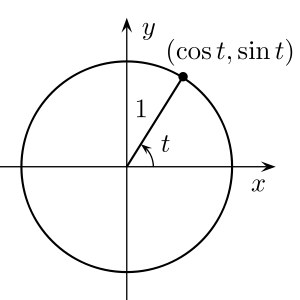
\includegraphics[scale=0.3]{complexcircle}
\end{center}

W dużym uproszczeniu okazuje się, że dodając do siebie odpowiednią ilość okręgów o odpowiedniednim promieniu otrzymuje się bazową funkcję/sygnał. Rozważając w ten sposób funkcję, czyli rozkładając bazowy sygnał na elementy, okazuje się, że ich badanie niesie ze sobą szereg zastosowań. 

\newpage

\section{Transformacja Fouriera}
Funkcja $f:  \mathbb{R}\rightarrow\mathbb{R}$ jest okresowa, o okresie $2T$ i całkowalna bezwzlgędnie w sensie Lebesque'a na całym \mathbb{R}. Załóżmy, że funkcja spełnia warunki Dirichleta w przedziale $[-T,T]$. Transformacja Fouriera jest przekształceniem liniowym, które funkcji $f(x)$ przyporządkowuje funkcję $F(u)$. Owe przekształcenia wyglądają następująco: \\

\begin{equation} \label{eu_eqn} \
f(x) = \frac{1}{\sqrt{2\pi}}\int_{-\infty}^{\infty}F(u)e^{-ixu}du
\end{equation}
Zatem:
\begin{equation} \label{eu_eqn} \
F(u) = \frac{1}{\sqrt{2\pi}}\int_{-\infty}^{\infty}f(t)e^{ixu}dt
\end{equation}

Na funkcję $f(x)$ oraz jej tranformatę $F(u)$ należy patrzeć jak na różne reprezentacje tej samej funkcji w różnych dziedzinach, na przykład w fizyce często spotyka się czas i częstotliwość jako jednostki zmiennych.

\section{Dyskretna transformacja Fouriera}
Ponieważ w praktyce wynikiem pomiarów są wartości dyskretne, konieczne stało się zdefiniowanie dyskretnej wersji ciągłej transformaty Fouriera. \\Dla $N$-elementowego ciągu $x_{n}$ dyskretną transformację Fouriera definiuje się następująco:


\begin{equation} \label{eu_eqn} \
\sum_{n=1}^{N-1} x_{n}e^{-\frac{2\pi i}{N}nk}, k \in {0, 1,...,N-1}
\end{equation}

DFT przekształca skończony ciąg próbek sygnału \newline $(a_{0}, a_{1}, a_{2},...,a_{N-1}), a_{i} \in \mathbb{R}$ w ciąg harmoniczny $(A_{0}, A_{1}, A_{2},...,A_{N-1}), A_{i} \in \mathbb{C}$. Ilość obliczeń jest następująca: $2N^2$, bo jest $N$ składników sumy (ze względu na n), jest $N$ równań (ze względu na k), wykonywane obliczenia to mnożenie liczb rzeczywistych przez zespolone. Liczenie dyskretnej transformaty Fouriera wymaga wysokiej mocy obliczeniowej, której komputery z lat 60-tych nie posiadały. W celu wykorzystania transformacji Fouriera J. Cooley i J. Tuckey opracowali szybszy algorytm transformowania.
\newpage

\section{Szybka Transformacja Fouriera}
W roku 1965 wyżej wspomniani matematycy opublikowali pracę pt. „An Algorithm for the machine computation of complex Fourier series”, gdzie opracowali szybki algorytm liczenia dyskretnej transformacji Fouriera (powszechnie FFT). FFT polega na zmniejszeniu liczby operacji DFT, w celu przyśpieszenia algorytmu. Klasyczną wersję dyskretnej transformacji można zapisać w postaci macierzowej: $\^s(0)$ jest wartością transformaty, a $s(0)$ jest wartością sygnału.
\begin{center}
    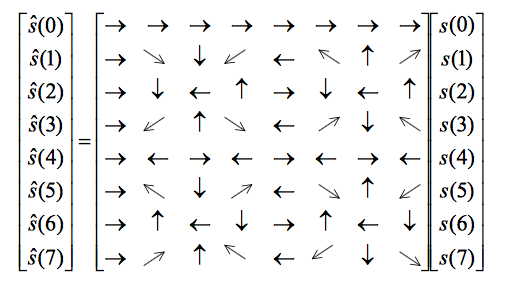
\includegraphics[scale=0.4]{sc1}        
\end{center}
\begin{center}
    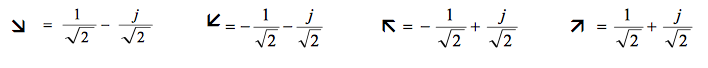
\includegraphics[scale=0.4]{cs3}        
\end{center}
Wynika stąd, że:
\begin{center}
    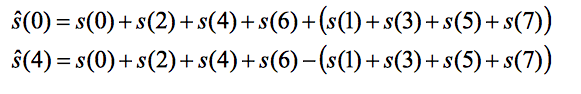
\includegraphics[scale=0.3]{sc2}
\end{center}
Okazuje się, że obliczenia są często dublowane. Celem uzyskania podobnego efektu jaki daje DFT, ale wykorzystującego mniej mocy obliczeniowej powstał algorytm FFT. Jeśli proces transformowania zostanie podzielony tak, żeby osobno liczy się próbki o numerach parzystych i osobno te o numerach parzystych ilość mnożeń wyniesie $N^2 + 2N$. FFT zakłada jednak lekko inne podejście, a mianowicie wielokrotne dzielenie próbek (operacja motylkowa). Wygląda to następująco:
\begin{center}
    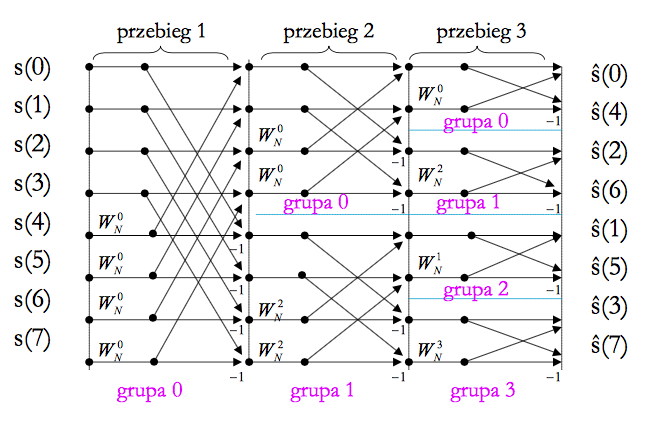
\includegraphics[scale=0.3]{sc4}
\end{center}
\newpage
Stosując taki podział próbek ilość operacji zmniejsza się do $N \log_{2} N$. Niżej znajduje się porównanie ilości operacji dla konketnej ilości danych wejściowych:
\begin{center}
    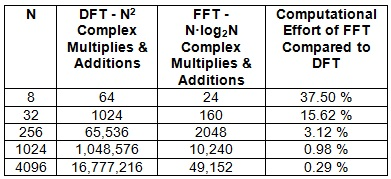
\includegraphics[scale=0.7]{sc5}
\end{center}
\begin{center}
    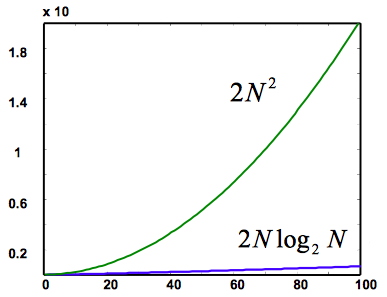
\includegraphics[scale=0.5]{sc6}
\end{center}

Źródła:
\begin{enumerate}


\item https://math.stackexchange.com/questions/1002/fourier-transform-for-dummies

\item Wykłady Analiza Matematyczna II dr. hab. Romana Wituły

\item Wykłady The Fourier Transforms and its Applications profesora Brad-a Osgood-a

\item http://main3.amu.edu.pl/~mcichon/tf.pdf

\item http://www.eetimes.com/document.asp?doc_id=1278838

\item https://upload.wikimedia.org/wikipedia/commons/thumb/8/8f/Unitcircle.svg/300px-Unitcircle.svg.png

\item https://pl.wikipedia.org/wiki/Dyskretna_transformata_Fouriera

\end{enumerate}


\end{document}
